\section{GPIO (General Purpose I/O)}

\subsection{GPIO Fundamentals}

\begin{definition}{GPIO}\\
    \begin{minipage}{0.5\linewidth}
    \textbf{Situation:}
    \begin{itemize}
        \item Microcontroller as a general purpose device
        \item Many functional blocks included
    \end{itemize}

    \textbf{Problem:}
    \begin{itemize}
        \item Limited number of pins
        \item Many functions to be implemented \\ (many functional blocks included)
    \end{itemize}
    \end{minipage}
    \begin{minipage}{0.5\linewidth}

    \textbf{Solution:}
    \begin{itemize}
        \item Many (all) pins are configurable as GPIO
        \item Select the needed I/O pins and functions
        \item \oq pin sharing\cq
        \item Output multiplexer needs to be configured
    \end{itemize}
    \end{minipage}
\end{definition}



\begin{minipage}{0.55\linewidth}
\begin{concept}{GPIO Overview}\\
General Purpose Input/Output (GPIO) pins allow the microcontroller to interact with the external world.
\begin{itemize}
    \item Pins can be configured as digital inputs or outputs
    \item Most pins support multiple functions (pin sharing) through internal multiplexers
    \item Configuration is done through memory-mapped registers
    \item Each GPIO port typically has 16 pins (e.g., GPIOA, GPIOB, etc.)
\end{itemize}
\end{concept}
\end{minipage}
\begin{minipage}{0.45\linewidth}
\begin{theorem}{Pin Sharing}
Multiple functions can share a single physical pin:
\begin{itemize}
    \item Digital inputs/outputs (GPIO)
    \item Serial interfaces (UART, SPI, I2C)
    \item Timers/Counters
    \item ADC (Analog-to-Digital Conversion)
    \item Alternate functions
\end{itemize}
Not all functions can be used simultaneously; configuration registers define pin usage.
\end{theorem}
\end{minipage}



\subsection{GPIO Structure}



\begin{concept}{Structure}\\
    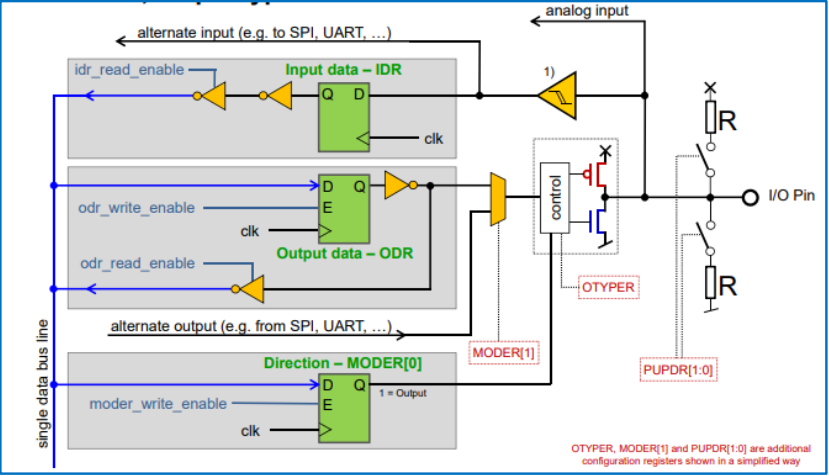
\includegraphics[width=\linewidth]{structure_gpio.png}
\end{concept}

\begin{corollary}{Push-Pull vs Open-Drain Outputs}

    \begin{minipage}{0.5\linewidth}
    \textbf{Push-Pull:}
    \begin{itemize}
        \item Can actively drive output high (to VDD) \\ or low (to GND)
        \item Faster switching times, can source and sink current
        \item Default output mode for GPIO pins
    \end{itemize}
    \end{minipage}
    \begin{minipage}{0.5\linewidth}
    \textbf{Open-Drain:}
    \begin{itemize}
        \item Can only actively drive output low
        \item Relies on external pull-up resistor to reach high state
        \item Multiple devices can share a line without conflicts (e.g., I2C bus)
        \item Used in "wired-AND" configurations
    \end{itemize}
    \end{minipage}
\end{corollary}

\columnbreak

\subsection{Data Registers and Operations}

\subsubsection{Register Access}

\begin{formula}{Register Address} = Base address + Offset
    \begin{itemize}
        \item Offset is given for each register in reference Manual
        \item Base address is defined in memory map (reference manual)
    \end{itemize}
\end{formula}

\begin{definition}{GPIO Registers}
Each GPIO port has several configuration registers:
\begin{itemize}
    \item \textbf{GPIOx\_MODER}: Mode register (input, output, alternate function, analog) - configures pin as input or output (direction control)
    \item \textbf{GPIOx\_OTYPER}: Output type register (push-pull or open-drain)
    \item \textbf{GPIOx\_OSPEEDR}: Output speed register (low, medium, high, very high) - configures speed
    \item \textbf{GPIOx\_PUPDR}: Pull-up/pull-down register
    \item \textbf{GPIOx\_IDR}: Input data register (read-only) - reads the pin state
    \item \textbf{GPIOx\_ODR}: Output data register (read/write) - sets the output state
    \item \textbf{GPIOx\_BSRR}: Bit set/reset register (atomic operations)
    \item \textbf{GPIOx\_LCKR}: Configuration lock register
    \item \textbf{GPIOx\_AFRL/H}: Alternate function registers (AF selection for pins 0-7 and 8-15)
\end{itemize}
\end{definition}

\begin{corollary}{Data Operations}
    \begin{itemize}
        \item Input: Read register \textbf{GPIOx\_IDR} (Input Data Register)
        \item Output: Write register \textbf{GPIOx\_ODR} (Output Data Register) or \textbf{GPIOx\_BSRR} (Bit Set Reset Register)
    \end{itemize}
\end{corollary}

\subsubsection{Hardware Abstraction Layer (HAL)}

\begin{definition}{HAL for GPIO}\\
The Hardware Abstraction Layer provides a structured way to access GPIO registers:
\begin{itemize}
    \item Based on structs that map to hardware registers
    \item Typedef for register structure (e.g., \texttt{reg\_gpio\_t})
    \item Pointers to each GPIO port (e.g., \texttt{GPIOA}, \texttt{GPIOB})
    \item Base addresses defined in header file
    \item Helper macros for bit manipulation
\end{itemize}
This approach makes code more readable and maintainable than direct register address manipulation.
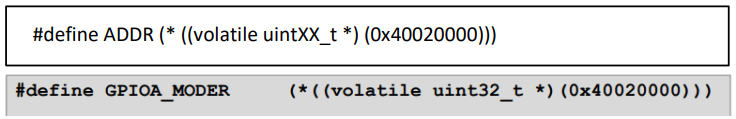
\includegraphics[width=0.7\linewidth]{HAL1.png}\\
    \textbf{Accessing a register:}
    \begin{itemize}
        \item each GPIO port has the same 10 registers 
        \item there are 11 GPIO ports $\rightarrow$ GPIOA to GPIOI
    \end{itemize}
\end{definition}

\begin{code}{Using HAL for GPIO}
\begin{lstlisting}[language=C, style=basesmol] 
// Using HAL style access
#include "reg_stm32f4xx.h"  // Contains structure definitions

// Configure PA3 as output
GPIOA->MODER &= ~(3 << 6);  // Clear bits 6-7
GPIOA->MODER |= (1 << 6);   // Set bit 6 (output mode)

// Instead of direct register access:
// volatile uint32_t *reg = (volatile uint32_t *)(0x40020000);
// *reg &= ~(3 << 6);
// *reg |= (1 << 6);
\end{lstlisting}
\end{code}

\begin{concept}{Hardware Abstraction Layer (HAL)}\\
    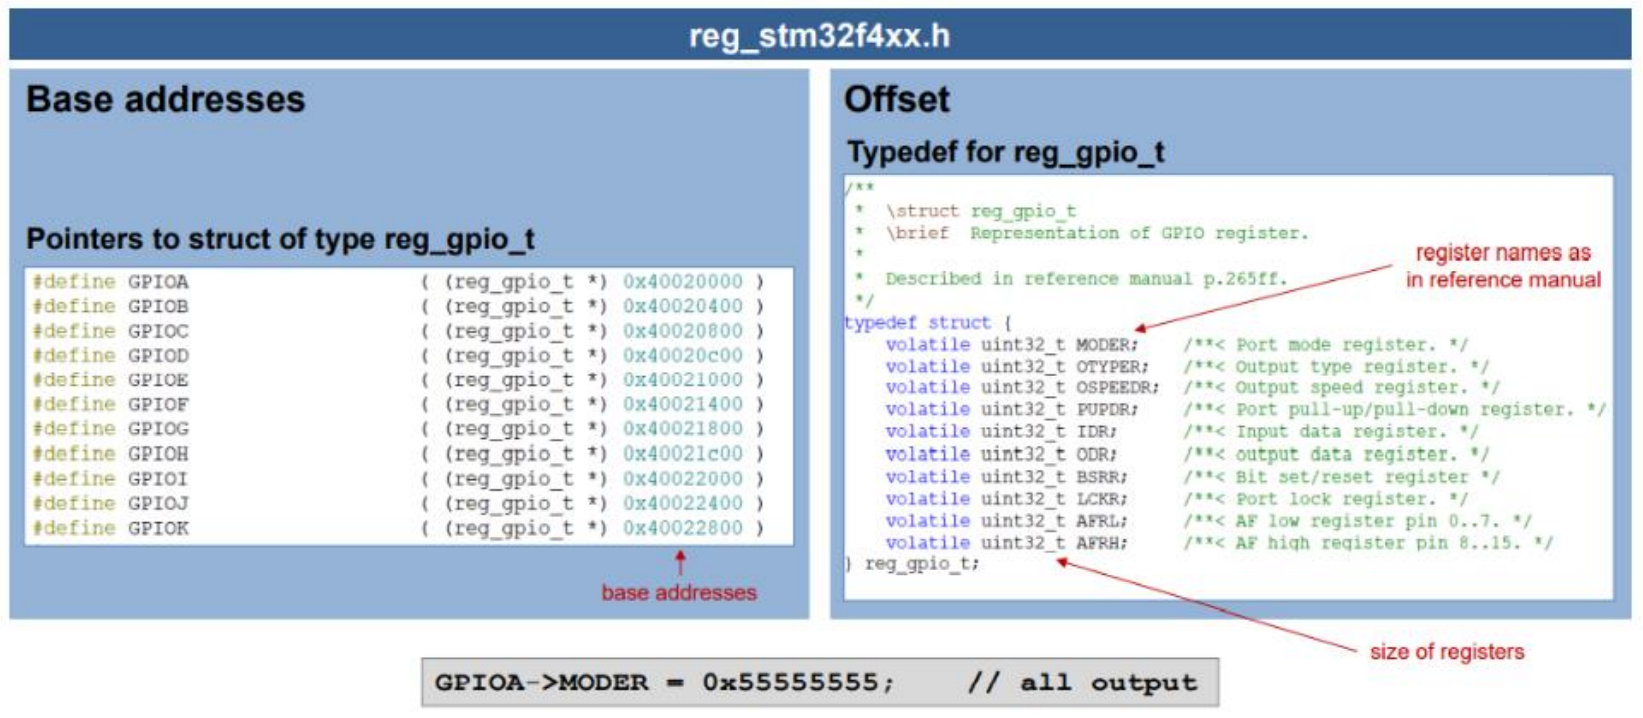
\includegraphics[width=\linewidth]{HAL2.png}
\end{concept}



\subsection{GPIO Configuration}

\important{SEP Handout: Datenblattauszug GPIO S.2-3 Addresses and Configurations}

\mult{2}

\begin{formula}{Input Data Register (IDR)}\\
The GPIOx\_IDR is a read-only register containing the input value of the corresponding I/O port.
\end{formula}

\begin{formula}{Direction Configuration (MODER)}\\
The GPIOx\_MODER register configures each pin's direction:
\begin{itemize}
    \item \textbf{00}: Input mode
    \item \textbf{01}: General purpose output mode
    \item \textbf{10}: Alternate function mode
    \item \textbf{11}: Analog mode
\end{itemize}
Each pin uses 2 bits in the register, allowing for 16 pins per port.
\end{formula}

\begin{formula}{Output Type (OTYPER)}\\
The GPIOx\_OTYPER register configures the output driver type:
\begin{itemize}
    \item \textbf{0}: Push-pull (can actively drive high or low)
    \item \textbf{1}: Open-drain (can drive low, relies on external pull-up for high)
\end{itemize}
\end{formula}

\begin{formula}{Pull-up/Pull-down (PUPDR)}\\
The GPIOx\_PUPDR register configures internal resistors:
\begin{itemize}
    \item \textbf{00}: No pull-up, no pull-down
    \item \textbf{01}: Pull-up
    \item \textbf{10}: Pull-down
    \item \textbf{11}: Reserved
\end{itemize}
\end{formula}

\begin{formula}{Output Data Register (ODR)}\\
The GPIOx\_ODR can be read and written to set the output state of GPIO pins.
\end{formula}

\begin{formula}{Speed Configuration (OSPEEDR)}\\
The GPIOx\_OSPEEDR register configures the output slew rate:
\begin{itemize}
    \item \textbf{00}: Low speed
    \item \textbf{01}: Medium speed
    \item \textbf{10}: High speed
    \item \textbf{11}: Very high speed
\end{itemize}
\end{formula}

\begin{formula}{Bit Set/Reset Register (BSRR)}\\
The GPIOx\_BSRR allows atomic bit operations:
\begin{itemize}
    \item Bits [15:0]: Set corresponding ODR bit by writing '1'
    \item Bits [31:16]: Reset corresponding ODR bit by writing '1'
\end{itemize}
This ensures atomic access without read-modify-write operations.
\end{formula}

\begin{KR}{Setting and Clearing Bits} GPIOx\_BSRR
    \begin{itemize}
        \item 0-15: Set Bits $\rightarrow$ 1: Set, 0: No Change
        \item 16-31: Reset/Clear Bits $\rightarrow$ 1: Reset, 0: No Change
        \item Ensures atomic access in software (no interruption possible)
    \end{itemize}
\end{KR}

\multend

\subsubsection{GPIO Configuration KR and examples}

\begin{KR}{Configuring GPIO Pins}
\paragraph{Identify GPIO port and pin}
\begin{itemize}
    \item Find the port letter (A-K) and pin number (0-15) from documentation
    \item Look up the corresponding pin number on the microcontroller package
\end{itemize}

\paragraph{Calculate register addresses}
\begin{itemize}
    \item Find the base address for the GPIO port in the memory map
    \item Calculate register addresses by adding offsets to the base address
    \item For STM32F4: Base addresses are at 0x4002 0000 + (0x400 * port\_index)
    \begin{itemize}
        \item GPIOA: 0x4002 0000
        \item GPIOB: 0x4002 0400
        \item GPIOC: 0x4002 0800
        \item And so on...
    \end{itemize}
\end{itemize}

\paragraph{Enable clock for GPIO port}
\begin{itemize}
    \item Use RCC\_AHB1ENR register to enable clock for the GPIO port
    \item Set the corresponding bit for the port
\end{itemize}

\paragraph{Configure specific pin properties}
\begin{itemize}
    \item Use GPIOx\_MODER to set pin mode/direction (input, output, alternate function, analog)
    \item Use GPIOx\_OTYPER to set output type (push-pull or open-drain)
    \item Use GPIOx\_OSPEEDR to set output speed (low, medium, high, very high)
    \item Use GPIOx\_PUPDR to configure pull-up/pull-down resistors
\end{itemize}

\paragraph{Set initial state (for outputs)}
For output pins, set the initial state in ODR or using BSRR.
\end{KR}


\begin{example2}{GPIO Configuration Exercise}
Configure pin PA3 as an output with open-drain configuration, low speed, and pull-up enabled. Then set the pin to low state.
\tcblower
First, identify the registers and their addresses:
\begin{itemize}
    \item GPIOA base address: 0x4002 0000
    \item GPIOA\_MODER: 0x4002 0000 (offset 0x00)
    \item GPIOA\_OTYPER: 0x4002 0004 (offset 0x04)
    \item GPIOA\_OSPEEDR: 0x4002 0008 (offset 0x08)
    \item GPIOA\_PUPDR: 0x4002 000C (offset 0x0C)
\end{itemize}

Then, calculate the bit fields for pin 3:
\begin{itemize}
    \item MODER3[1:0] = 01 (output mode) at bits 7:6
    \item OTYPER3 = 1 (open-drain) at bit 3
    \item OSPEEDR3[1:0] = 00 (low speed) at bits 7:6
    \item PUPDR3[1:0] = 01 (pull-up) at bits 7:6
\end{itemize}

\begin{lstlisting}[language=C, style=basesmol] 
// Enable GPIOA clock
RCC->AHB1ENR |= (1 << 0);  // Bit 0 for GPIOA
// Configure PA3 as output (bits 6-7 = 01)
GPIOA->MODER &= ~(3 << 6);  // Clear bits 6-7
GPIOA->MODER |= (1 << 6);   // Set bit 6 (output mode)
// Configure as open-drain (bit 3 = 1)
GPIOA->OTYPER |= (1 << 3);  
// Configure as low speed (bits 6-7 = 00)
GPIOA->OSPEEDR &= ~(3 << 6);  // Clear bits 6-7 (low speed)
// Configure with pull-up (bits 6-7 = 01)
GPIOA->PUPDR &= ~(3 << 6);    // Clear bits 6-7
GPIOA->PUPDR |= (1 << 6);     // Set bit 6 (pull-up)
// Set pin to low state using BSRR
GPIOA->BSRR = (1 << (3 + 16));  // Set bit 19 (reset PA3)
// or using ODR
GPIOA->ODR &= ~(1 << 3);  // Set PA3 low
\end{lstlisting}
\end{example2}

\begin{KR}{Reading and Writing GPIO}
\paragraph{Reading Input Pins}
Read the current state of GPIO pins using the IDR register.
\paragraph{Writing Output Pins - Using ODR}
Set or clear output pins by modifying the ODR register.
\paragraph{Writing Output Pins - Using BSRR (preferred)}
Set or clear output pins atomically using the BSRR register.

\begin{lstlisting}[language=C, style=basesmol] 
// Reading input from GPIOA pin 0
uint32_t buttonState = (GPIOA->IDR & (1 << 0)) != 0;

// Writing output using ODR (not atomic)
// Set pin high
GPIOA->ODR |= (1 << 5);
// Set pin low
GPIOA->ODR &= ~(1 << 5);

// Writing output using BSRR (atomic)
// Set pin high (bits 0-15)
GPIOA->BSRR = (1 << 5);
// Set pin low (bits 16-31)
GPIOA->BSRR = (1 << (5 + 16));
\end{lstlisting}
\end{KR}

\begin{example2}{GPIO LED und Button Konfiguration}\\
    STM32F429 Discovery Board:
    \begin{itemize}
        \item User Button B1: GPIO Port A, Pin 0
        \item User LED LD3 (grün): GPIO Port G, Pin 13
        \item User LED LD4 (rot): GPIO Port G, Pin 14
    \end{itemize}
    
    Konfiguriere Pin 13 als Output mit Open-Drain und Pull-up.
    
    \tcblower
    
    \textbf{Register und Adressen:}
    \begin{itemize}
        \item GPIOG\_MODER: 0x40021800
        \item GPIOG\_OTYPER: 0x40021804
        \item GPIOG\_OSPEEDR: 0x40021808
        \item GPIOG\_PUPDR: 0x4002180C
    \end{itemize}
    
    \textbf{Bit-Konfiguration für Pin 13:}
    \begin{itemize}
        \item MODER[27:26] = 01 (Output Mode)
        \item OTYPER[13] = 1 (Open-Drain)
        \item OSPEEDR[27:26] = 01 (Medium Speed)
        \item PUPDR[27:26] = 01 (Pull-up)
    \end{itemize}
    
    \textbf{C-Code:}
\begin{lstlisting}[style=basesmol]
// LED ein-/ausschalten mit BSRR
// LED einschalten (Pin 13)
GPIOG->BSRR = (1 << 13);

// LED ausschalten (Pin 13)
GPIOG->BSRR = (1 << (16+13));

// Button lesen (Pin 0)
uint32_t button_state = GPIOA->IDR & 0x1;
\end{lstlisting}
\end{example2}

\begin{remark}
    Das BSRR (Bit Set/Reset Register) ermoeglicht atomare Bit-Operationen. Die unteren 16 Bits (0-15) setzen die entsprechenden Pins, die oberen 16 Bits (16-31) loeschen die entsprechenden Pins (Bit 16 loescht Pin 0, Bit 17 loescht Pin 1, etc.).
\end{remark}

\raggedcolumns
\columnbreak




\begin{KR}{Using GPIO Data Registers}
\paragraph{Reading input pins}
\begin{itemize}
    \item Use GPIOx\_IDR register to read the state of input pins
    \item Bit n corresponds to pin n (0-15)
    \item Apply appropriate bit mask to extract the bit(s) of interest
\end{itemize}

\paragraph{Writing output pins}
\begin{itemize}
    \item Use GPIOx\_ODR register to write to output pins
    \item Bit n corresponds to pin n (0-15)
    \item Writing to ODR affects all bits at once, which can lead to race conditions
\end{itemize}

\paragraph{Atomic bit manipulation}
\begin{itemize}
    \item Use GPIOx\_BSRR register for atomic bit setting/clearing:
    \begin{itemize}
        \item Bits 15:0: Setting corresponding ODR bits (write 1 to set)
        \item Bits 31:16: Clearing corresponding ODR bits (write 1 to clear)
    \end{itemize}
    \item Example: To set pin 5, write (1 << 5) to BSRR
    \item Example: To clear pin 5, write (1 << (16+5)) to BSRR
\end{itemize}
\end{KR}

\begin{example2}{GPIO Data Operations Example}\\
Write code to:
\begin{enumerate}
    \item Read the state of user button B1 on port A, pin 0
    \item Turn on the green LED LD3 on port G, pin 13 when B1 is pressed
    \item Turn on the red LED LD4 on port G, pin 14 when B1 is not pressed
\end{enumerate}

\tcblower
First, define the register addresses and pin mappings:

\begin{lstlisting}[language=C, style=basesmol]
// Button B1 is on PA0
// Green LED LD3 is on PG13
// Red LED LD4 is on PG14

#include "reg_stm32f4xx.h"

void button_led_control(void) {
    // Read button state (PA0)
    uint32_t button_state = GPIOA->IDR & (1 << 0);
    
    if (button_state) {
        // Button pressed - turn on green LED (PG13) and turn off red LED (PG14)
        // Set bit 13, clear bit 14 atomically
        GPIOG->BSRR = (1 << 13) | (1 << (16+14));
    } else {
        // Button not pressed - turn on red LED (PG14) and turn off green LED (PG13)
        // Set bit 14, clear bit 13 atomically
        GPIOG->BSRR = (1 << 14) | (1 << (16+13));
    }
}
\end{lstlisting}

Note: This assumes that the GPIO ports have been properly configured:
\begin{itemize}
    \item PA0 (Button B1) as input with pull-up/pull-down as needed
    \item PG13 (LED LD3) as push-pull output
    \item PG14 (LED LD4) as push-pull output
\end{itemize}
\end{example2}